\section{Speaker Independence}
\label{sect:speaker-independence}
Normal TDNNs are time invariance. However men, women and children differ in \textit{frequency}. Men normally have a darker voice than women and children. Therefore we have to compensate this invariance.


Observations on TDNNs
\begin{itemize}
	\item TDNNs develope linguistically plausible features in the hidden units
	\item TDNNS developed alternate internal representations that can link quite different acoustic realizations to the same higher level concept (because of multilayer arrangement)
	\item hidden units fire synchrony because they operate independent of precise time alignment or segmentation (time invariant)
	\item small network output may not be useful in complex task (but the internal abstractions may be valuable)
	\item complex concepts -> use stages with different knowledge
	\item new learning strategies should be build in existing knowledge
\end{itemize}
Model invariance
\begin{itemize}
	\item frequency shift, tilt, compression
\end{itemize}
Variability
\begin{itemize}
	\item adaption
		\begin{itemize}
			\item slow adaption -> modify weights
			\item fast adaption -> pretrained specific submodels
		\end{itemize}
	\item normalization
		\begin{itemize}
			\item environment: to the room
			\item speaker: mapping new speaker to standard speaker (with standard sentences)
		\end{itemize}
\end{itemize}
Combine \textbf{two standard TDNNs} to one (overall better classification): one with MSE and the other with CFM. Those combination yields the correct classification.\\
Even better than two TDNNs: \textbf{three TDNNS}! The third TDNN uses CE.

\subsection{Frequency Invariance}
\label{ssect:frequency-invariance}
\textit{Convolutional Acoustic Models}:
\begin{itemize}
	\item parameter sharing across spectrum and time -> exploit 2D structure of features
	\item upper layer fully connected
	\item pooling gives more robustness and less overfitting
\end{itemize}

\subsection{Multi-Speaker Reference Model}
\label{ssect:multi-speaker-reference-model}
Idea: A speaker-specific reference model is composed from several well trained reference models:
\begin{figure}[h]
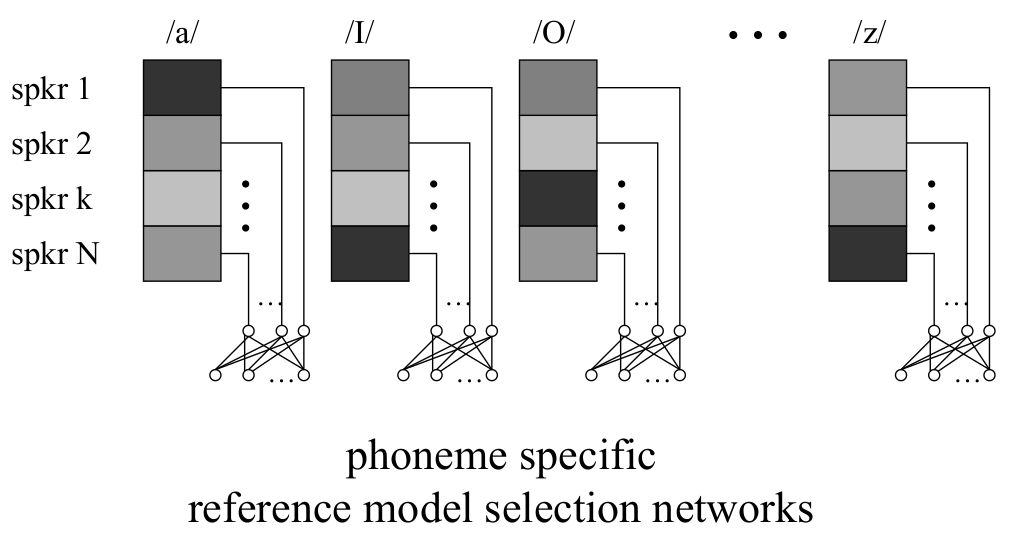
\includegraphics[scale=0.4]{phoneme-specific-reference-model-selection-networks}
\end{figure}\\
Meta-Pi-Net:
\begin{figure}[h]
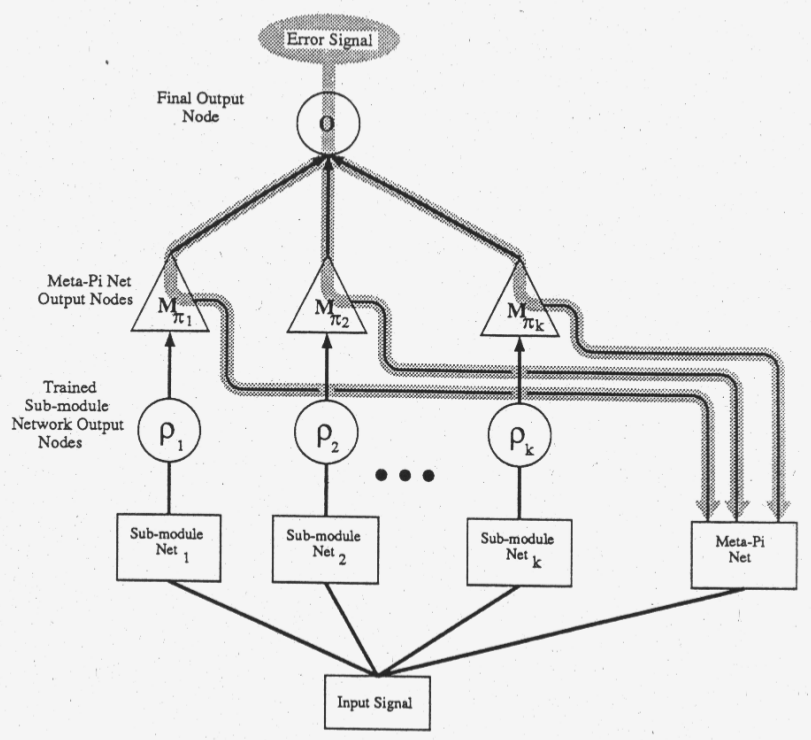
\includegraphics[scale=0.4]{meta-pi-model}
\end{figure}\\
A seperate neural net \textit{Meta-Pi-Net} controls the activation / deactivation of the single nets. The whole net is a combination of one net per speaker. In general we look which speaker net is closest to the input (which nets classifies the best). The Meta-Pi-Net produces weights for each net which control how much each net is taking into account for the classification.\\
It is not important that the correct speaker is chosing. Sometimes a combination of two or more speaker might fit better to the input. The actual correct speaker net might not be even taking into account (results in a mixture of the other nets).\\[1cm]

\textbf{Speaker Normalization}: we have speaker dependent nets. Now when we use those nets to classifier what another speaker says (no dependent net for this speaker!) the error rate is 41.9\%. With 40 text-dependent training sentences the error rate is reduced to 6.8\%.

\textbf{i-vectors}: identity vectors (i-vectors) describe the speaker-characteristic offset to an universal background model. Those i-vecotrs are used to train a recognition system.\\[1cm]

\textit{Speaker Adaptive Training of DNN}:
\begin{itemize}
	\item[1.] train initial DNN with (and keep it fixed)
		\begin{itemize}
			\item SI features: fbank
			\item SA features: Feature space Maximum Likelihood Linear Regression (fMLLR)
		\end{itemize} 
	\item[2.] Train an i-vector NN
		\begin{itemize}
			\item inputs: i-vectors
			\item outputs: linear shift to the original feature vectors
			\item added features become speaker-normalized
		\end{itemize}
	\item[3.] update the DNN in the new feature space, i-vector NN fixed -> yields SAT-DNN
\end{itemize}

\subsection{Cross-Language DNNs}
\label{ssect:cross-language-dnns}
\textit{Multilingual Bottleneck Features}:
\begin{itemize}
	\item Humans can only produce a finite amount of different sounds
	\item Subset of sounds is used in individual languages
	\item Some sounds are used in different languages
	\item Share data of the same sounds from different languages
	\item Extract more robust features using data with more variability
\end{itemize}
\begin{figure}[h]
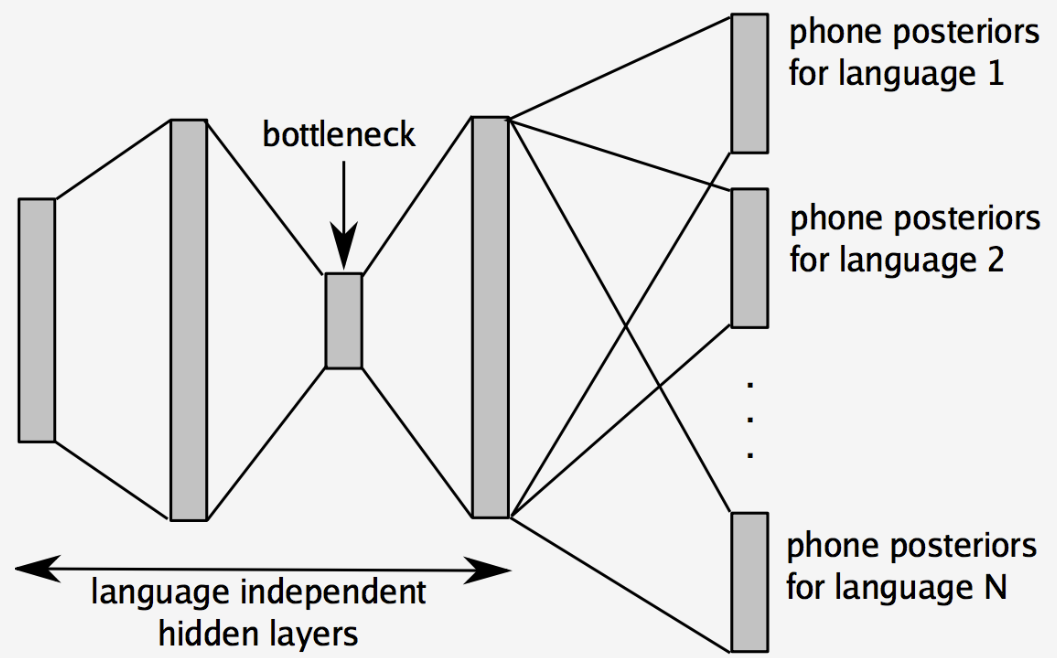
\includegraphics[scale=0.4]{multilingual-bottleneck-features}
\end{figure}
Cross-Language DNNs with Language-Universal Feature Extractors:
\begin{figure}[h]
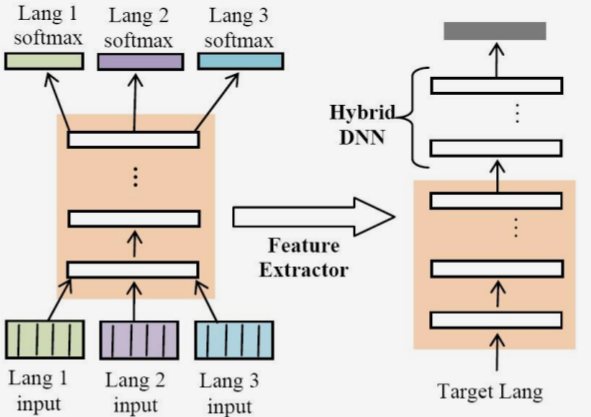
\includegraphics[scale=0.4]{DNNs-LUFE}
\end{figure}\\
DNNs can be trained on mutltiple languages. The hidden layers (\textit{language-universal feature extractor}) are used in other DNNs.

\newpage